\documentclass[a4paper,10pt]{article}
\usepackage[utf8]{inputenc}
\usepackage{graphicx}
\usepackage{url}
\usepackage{float}
\usepackage{times}
\usepackage{multirow}
\usepackage{listings}
\usepackage{times}
\usepackage{paralist}
\usepackage{epsfig}
\usepackage{subfigure}
\usepackage[hypertex]{hyperref}
\usepackage{subfigure}
\usepackage{color}
\usepackage{xspace}

%\documentclass{rspublic}

\usepackage{ifpdf}

\newcommand{\I}[1]{\textit{#1}}
\newcommand{\B}[1]{\textbf{#1}}
\newcommand{\BI}[1]{\textbf{\textit{#1}}}
\newcommand{\T}[1]{\texttt{#1}}

\newcommand{\sagaspec}{\textit{SAGA}\xspace}
\newcommand{\sagaimpl}{\textit{SAGA}\xspace}

\newcommand{\spec}{\sagaspec}
\newcommand{\impl}{\sagaimpl}

\setlength\topmargin{0in}
\setlength\headheight{0in}
\setlength\headsep{0in}
\setlength\textheight{9.5in}
\setlength\textwidth{6.5in}
\setlength\oddsidemargin{0in}
\setlength\evensidemargin{0in}
\setlength\parindent{0.1in}
\setlength\parskip{0.25em}


\ifpdf
 \DeclareGraphicsExtensions{.pdf, .jpg}
\else
 \DeclareGraphicsExtensions{.eps, .ps}
\fi

\newcommand{\note}[1]{ {\textcolor{red} { ***NOTE: #1 }}}

\newif\ifdraft
\drafttrue

\ifdraft
\newcommand{\amnote}[1]{   {\textcolor{magenta} { ***Andre:    #1 }}}
\newcommand{\jhanote}[1]{  {\textcolor{red}     { ***Shantenu: #1 }}}
\else
\newcommand{\amnote}[1]{}
\newcommand{\jhanote}[1]{}
\fi

\begin{document}

 \title{  \vspace{-3.5em}	SAGA AHM 2010 - Needs Title}
 
 \author{Shantenu Jha$^{1,2,3}$, Hartmut Kaiser$^{1}$, Andre Merzky$^{1}$, Ole Weidner$^{1}$ \\
   \small{\emph{$^{1}$Center for Computation \& Technology, Louisiana State University, USA}}\\
   \small{\emph{$^{2}$Department of Computer Science, Louisiana State University, USA}}\\
   \small{\emph{$^{3}$e-Science Institute, University of Edinburgh, UK}}
 }
 \date{}
 \maketitle
 

 \jhanote{Remember in addition to serving as an abstract, this will
   serve as a summary of what will go to the 3 editors of the journals
   that we are considering publishing a full paper in. Thus some more
   information/discussion on what the underlying problem and context
   will be about.}


 \jhanote{Once we have defined / introduced SAGA, we should probably
   have 3 subsections -- interface, library and adatptors/backends?}

\subsection*{A Powerful, Community-Driven Standard}

 The \spec API evolved from within several early grid adopter
 communities, which perceived the need of a uniform and simple
 programmatic interface that would be widely-adopted and
 widely-available.  The goal of such an interface is to provide a
 ``distributed computing counterpart to MPI'' (at least in impact, if
 not in details), and to supply developers with a simple, uniform, and
 standard (i.e. stable) programmatic interface with which to develop
 applications.  The scope and requirements of the \spec API is
 formally defined by OGF's SAGA Working Group (SAGA-WG), and were
 derived from use cases collected from a broad user community (see
 GFD.70~\cite{ogf-gfd-70} and GFD.71~\cite{ogf-gfd-71}).  The result
 of this process is the version 1.0 of the \spec Core API
 specification (GFD.90~\cite{ogf-gfd-90}), which defines the \spec
 Core (including error handling, session management, monitoring and
 notfication, and asynchronous operations) and several functional API
 packages (jobs, name-spaces, files, replicas, streams, rpc) in a
 language independent way.  Additional API extension packages, such as
 CPR (GWD-R.96~\cite{ogf-gwd-r-96}), Adverts
 (GFD-R-P.XX~\cite{ogf-gwd-r-p-xx}), and Messages
 (GWD-R.94~\cite{ogf-gwd-r-94}) are currently under development and
 follow a similar, well-defined community-driven standardization and
 approval process. \spec is now an Open Grid Forum (OGF)~\cite{ogf}
 proposed recommendation on the path to becoming a full standard in
 2010.  The standardization is not important in and of itself, but
 rather because it makes it more likely that other infrastructures
 will also support \spec, which makes it, in essence, a de facto
 standard for users of most national CI projects.


\subsection*{A Modular and Extensible Architecture}

The \impl \I{Core Components} and \I{Adaptors} an implementation
of the \spec API Specification written in C++ and Python. \impl is
Open Source software, released under the Boost Software
License 1.0~\cite{boost_license_web}. It can be divided into
three major components (as depicted in Fig. \ref{fig:saga_arch}):
the \I{Core Components} which provide the API functionality, the
\I{Adaptors} which translate API calls into native middleware calls,
the Python API \I{Language Bindings} and a set of \I{Command Line
  Tools}. The \impl \I{Core Components} are a collection of dynamic
libraries and header files that represent the functional API packages
(see section 2.1) along with a lightweight, highly-configurable
\I{Engine Component} that manages call dispatching and the dynamic
runtime loading of the \I{Middleware Adaptors}.


Each of these \I{Adaptors} implements the functionality of a specific
functional package (e.g., job adaptors, file adaptors) for a specific
middleware system. Adaptors are also realized as dynamic
libraries. \impl provides adaptors for many grid and distributed
computing middleware, including the Globus Toolkit, Condor, Platform
LSF and Amazon EC2. Several other adaptors, notably adaptors for PBS,
gLite and BES are under development. The Python API \I{Language
  Bindings} are an optional component of \impl that adds a thin Python
layer on top of the native C++ API. This simple but very popular
component allows application developers to quickly prototype and
implement \impl-based applications in Python.  The layered, decoupled
architecture of \impl allows for maximum flexibility at compile and
runtime. It allows the user of to freely and selectively combine the
library components and easily develop additional components orthogonal
to the existing ones. More details on \impl's architecture and its
implementation details can be found in \cite{OOPSLA_PAPER}.

%  The forth and last
% component are the \I{Command Line Tools}. They provide a
% non-programmatic access to each of \impl's functional packages: the
% \I{file tool} provides access to file operations, like read, copy,
% delete, move, etc., the \textit{job tool} allows simple submission and
% control ofcompute jobs, and so on.


\subsection*{A Mature Software Engineering Process\label{engineering}}

The \impl engineering process is closely supervised by the technical
project manager. It follows an iterative and incremental model in
which the evaluation and learning phase is strongly community
driven. \impl provides independent releases for the \I{Core
  Components}, the \I{Language Bindings} and the \I{Adaptors}, which
provides maximum flexibility and short shortest reaction times for
bugfix-releases. All releases are available on the saga
website~\cite{saga_downloads_web} and are fed into a very responsive
community of users, which subsequently files bugs and suggests
improvement through a central ticket
system~\cite{saga_bugtracking_web} which is tightly integrated into
the development process. These reports along with strategic long-term
development goals form the requirements for the next
iteration. Individual developers are usually responsible for specific
components over the component's whole lifetime. This does not only
ensure clearly defined targets for task assignments, but also results
in growing expertise and specialization for the individual
developers. The core \impl development team has been working together
for more than three years and has evolved into a very smooth running
operation. Nevertheless, the \impl development process is completely
open: community involvement is not only accepted but encouraged and
has lead to successful collaborations and enrichment of the \impl
landscape in the past.

Along with the development of \impl, we maintain and constantly extend a broad set of unit and conformance tests to verify proper functioning and to validate OGF standard compliance. Most of the tests are written on a per-package basis using the Boost Test library~\cite{boost_test_web} and Python's built-in unit test framework. To facilitate the continuous integration (CI) aspect in the \impl development process, all tests are run constantly and automated using an automated CI rig\cite{buildbot_web} which provides feedback for every single change in the saga source tree. This way build problems and failing tests are pinpointed quickly and the responsible developer can take action. These automated tests are  our most valuable tool for early error and bug detection and has lead to a constantly higher quality of our releases since its introduction.
 
%\subsection*{A Strong and Diverse Application Community}

\subsection*{SAGA: Sustainability}

\subsection*{Addressing the needs of the e-Science Community}
\jhanote{SJ Will write} \note{Shantenu's playground: talk about
  scientific applications using saga directly (...), talk about CS
  people taking saga and use it to build higher-level frameworks and
  tools (faust, bigjob, diggedag...). The usual stuff ;-)}

SAGA is being used by a broad set of users in many different ways --
both to support production-grade science as well as to facilitate
research into distributed systems and applications.  For applications,
the most common mode of uptake has been in the development of
``frameworks'' -- logical compoments that meet specific application
requirements. Some specific examples of such frameworks, include the
Pilot-Job Framework (BigJob) and a self-adapting computing framework
(Lazarus); other frameworks are based upon generalisations of well
known patterns such as All-Pairs. SAGA-based frameworks support a
wide-range of scientific activity, ranging from the Virtual
Physiological Human (VPH) to Resorvoir simulations hierarchichal
molecular dynamics simulations on the TeraGrid.

Another common mode of SAGA usage is the creation of tools that are
extensible and work over different infrastructure. Once again,
SAGA-based tools are being utilised for production-grade as well as
research-prototyping. Prominent examples of the former, include the
GANGA-DIANE toolset, JSAGA, NAREGI job submission/management
system. Examples of research prototypes include digedag -- an
experimental system to support the flexible execution of DAG-based
workflow applications.

Finally, several applications (e.g., numerical relativity
applications) have used SAGA directly to support remote job submission
and file/date transfer. Although this was an initial target usage
mode, the cumulative number of such users is less than the previous
two modes. It is worth mentioning that applications typically tend to
use SAGA directly in early (fast-track) stages, but then move to
deeper integration via frameworks.

\pagebreak

\begin{figure}[hb]
  \centering
  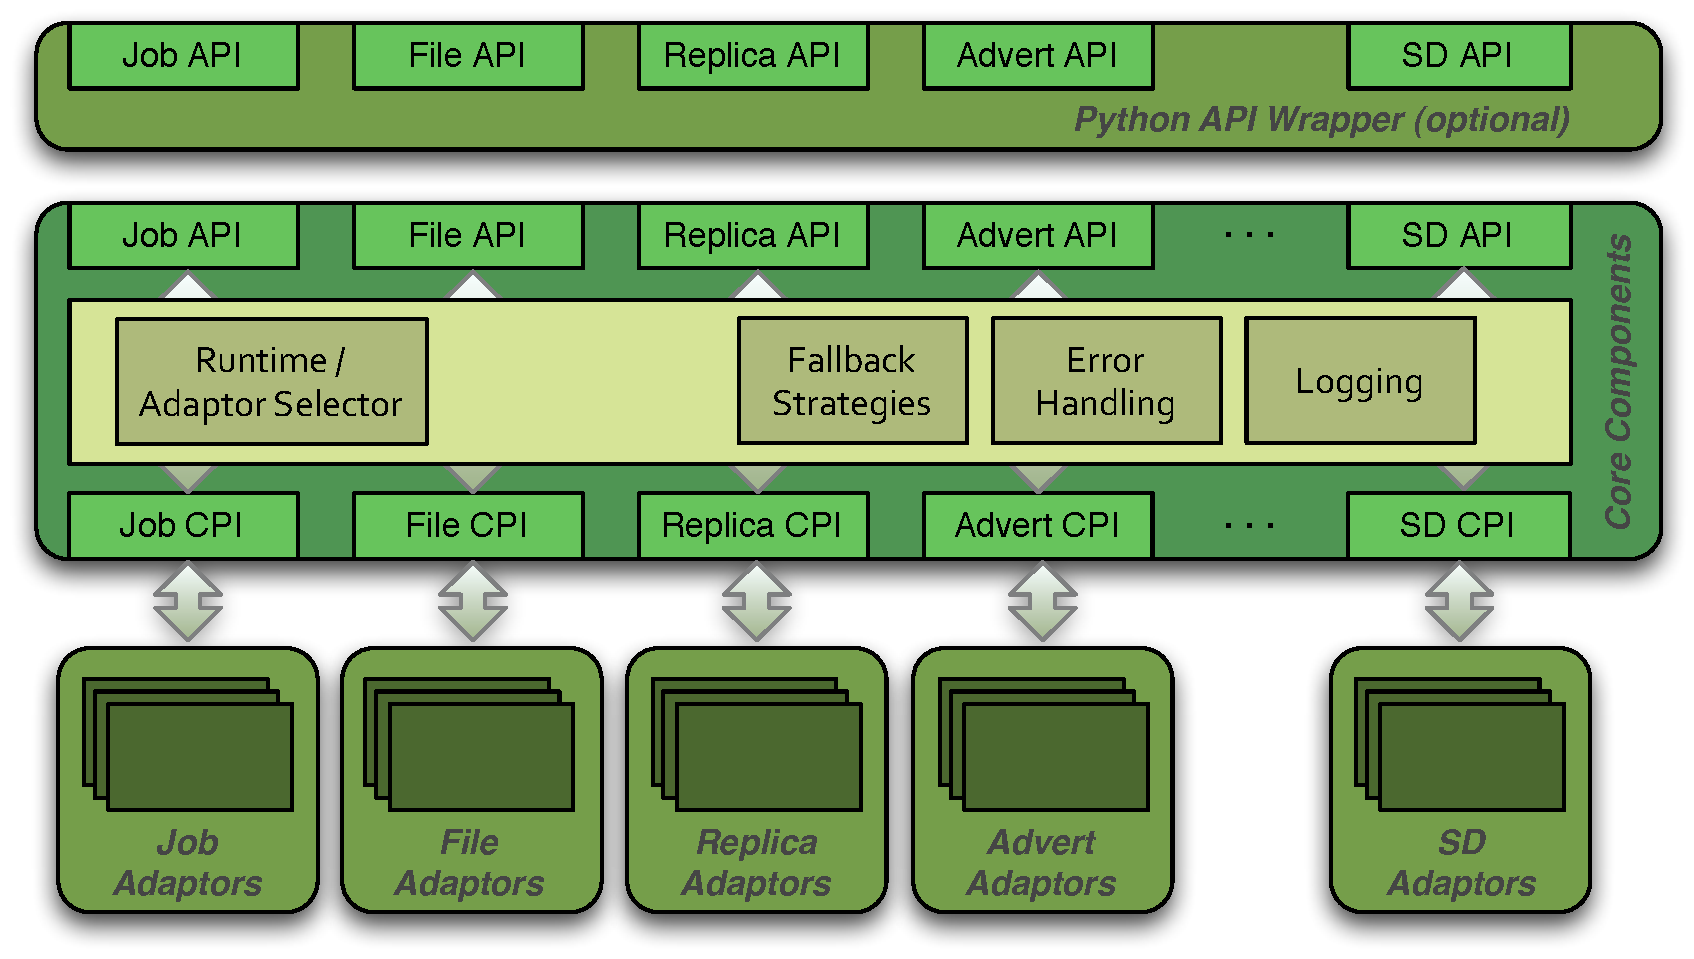
\includegraphics[width=4in]{./figures/saga-architecture}
 \vspace{-1em}	
  \caption{\footnotesize Layered schematic of the different
    components of \impl.  Middleware specific adaptors make
    applications developed using \impl portable.  Schematic showing
    the different ways in which \impl can be used to develop
    distributed applications. (i) Using native \impl calls to
    implement distributed functionality; (ii) Through the use of
    frameworks which provide either application-level usage modes,
    patterns and thus shielding the application from directly
    interfacing with the infrastructure.}
%\vspace{-1.5em}
  \label{fig:saga_arch}
\end{figure}

 \bibliographystyle{IEEEtran} 
 \bibliography{saga_ahm_abstract}


\end{document}

